\documentclass{beamer}

\usepackage{comment}
\usepackage{color}
\usepackage{listings}
\usepackage{verbatim}
\usepackage{multicol}
\usepackage{booktabs}
\usepackage{textpos}
\usepackage{graphicx}
\usepackage{graphics}
\definecolor{green}{RGB}{0,128,0}

\newcommand\gehcomment[1]{{{\color{orange} #1}}}
\newcommand\add[1]{{{\color{blue} #1}}}
\newcommand\remove[1]{\sout{{\color{red} #1}}}
\newcommand\codecomment[1]{{{\color{green} #1}}}
\newcommand\redcomment[1]{{{\color{red} #1}}}
\newcommand\bluecomment[1]{{{\color{blue} #1}}}
\newcommand\greencomment[1]{{{\color{green} #1}}}
\newcommand\magentacomment[1]{{{\color{magenta} #1}}}

\begin{document}
\title{1D Buoyant Flow\ldots}
\author{Michael Nole}
\date{\today}

%\frame{\titlepage}

%-----------------------------------------------------------------------------
\section{Description of 1D Buoyant Flow Scenario}

\subsection{1D Buoyant Flow Conceptual Model}

\frame{\frametitle{Description of 1D Buoyant Flow Scenario}

The ``1D Buoyant Flow Scenario'' simulates vertical migration of free-phase CO2 in a 1D fracture. This scenario demonstrates the basics of setting up an input deck with gravity, checkpointing, and restarting simulations using \bluecomment{SCO2 MODE}.

This demonstration covers the following:

\begin{itemize}
  \small
  \item Set up a 1D vertical model using SCO2 mode.
  \item Run the simulation to steady state.
  \item Modify initial and boundary conditions to simulate vertical flow of CO2.
  \item Run the simulation, visualize results.
\end{itemize}
}

%-----------------------------------------------------------------------------
\section{Description of Input Deck}

%-----------------------------------------------------------------------------
\subsection{DESCRIPTION}

\begin{frame}[fragile,allowframebreaks]\frametitle{DESCRIPTION}

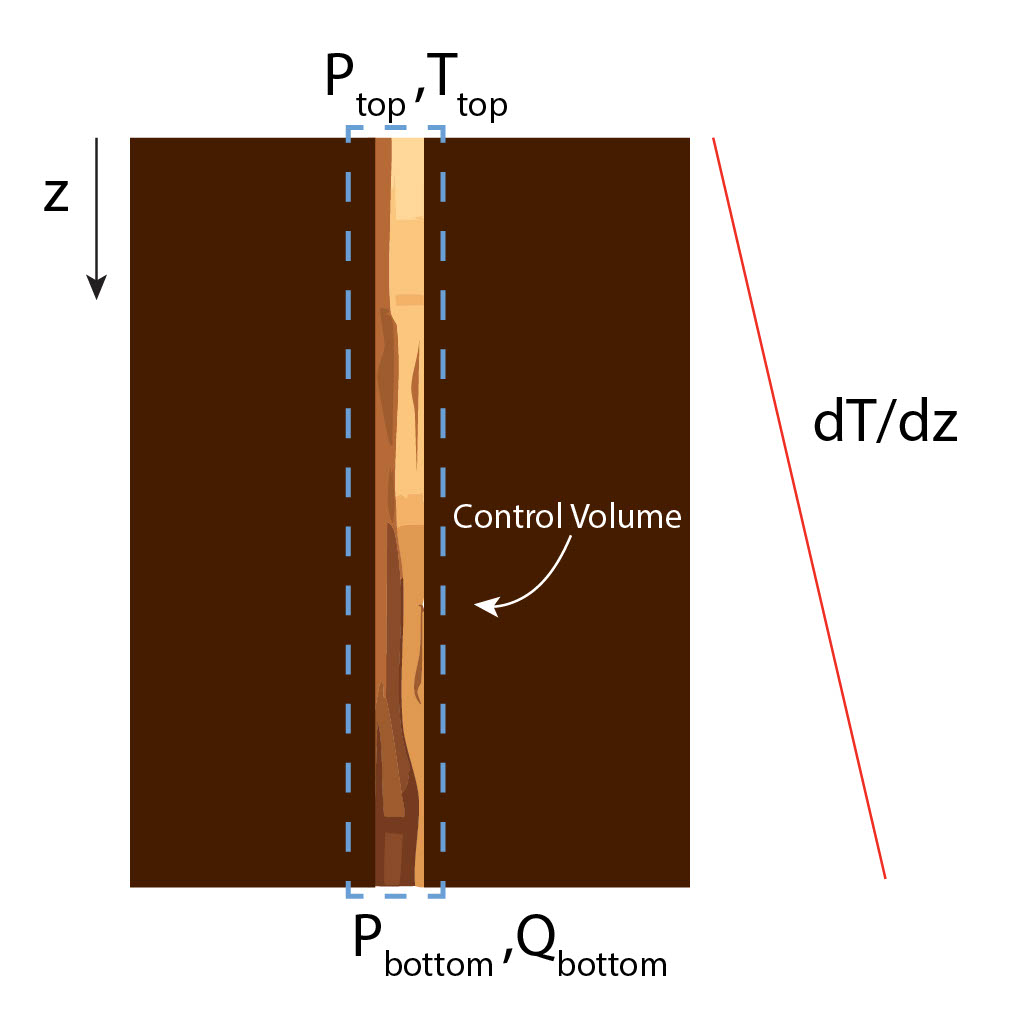
\includegraphics[height=3in]{buoyant_flow_fig.jpg}

\newpage
\begin{itemize}
  \item 1. Initialize with hydrostatic pressure and geothermal gradient
  \item 2. Apply constant heat flux
  \item 3. Run to steady state
  \item 4. Restart simulation with pressurized CO2 bottom BC
\end{itemize}

\end{frame}

%-----------------------------------------------------------------------------
\subsection{SIMULATION\_BUOYANT\_FLOW\_INITIAL}

\begin{frame}[fragile]\frametitle{SIMULATION: Buoyant Flow (Initial)}

\begin{itemize}
\item Specify SCO2 flow mode
\item Add checkpointing
\end{itemize}


\begin{semiverbatim}
SIMULATION
  SIMULATION_TYPE SUBSURFACE
  PROCESS_MODELS
    SUBSURFACE_FLOW flow
      MODE SCO2
    /
  /
CHECKPOINT
  FORMAT HDF5
/
END

SUBSURFACE
...

\end{semiverbatim}

\end{frame}

%-----------------------------------------------------------------------------
\subsection{NUMERICAL METHODS}
\begin{frame}[fragile]\frametitle{NUMERICAL METHODS}

\begin{itemize}
  \item Numerical Methods within subsurface block
  \item Newton Solver and Linear Solver sub-blocks
\end{itemize}

\begin{semiverbatim}
NUMERICAL_METHODS flow

  NEWTON_SOLVER
    USE_INFINITY_NORM_CONVERGENCE
    NUMERICAL_JACOBIAN
  END

  LINEAR_SOLVER
    SOLVER DIRECT
  END

  TIMESTEPPER flow
    TIMESTEP_MAXIMUM_GROWTH_FACTOR 1.25d0
  END

END

\end{semiverbatim}
\end{frame}
%-----------------------------------------------------------------------------
\subsection{GRID}
\begin{frame}[fragile,containsverbatim]\frametitle{GRID}

\begin{itemize}
  \item Cartesian grid
  \item Gravity points downward
\end{itemize}

\begin{semiverbatim}
GRID
  TYPE STRUCTURED CARTESIAN
  GRAVITY 0.d0 0.d0 -9.81d0
  NXYZ 1 1 100
  DXYZ
    25.d0
    1@1.d0
    100@5.d0
  /
END
\end{semiverbatim}

\end{frame}
%-----------------------------------------------------------------------------
\subsection{FLUID\_PROPERTIES}
\begin{frame}[fragile,containsverbatim,allowframebreaks]\frametitle{Fluid Properties}

\begin{itemize}
  \item Define properties of water and gas
  \begin{itemize}
    \item Diffusion coefficients
    \item Equations of state
  \end{itemize}
\end{itemize}

\begin{semiverbatim}
FLUID_PROPERTY
  PHASE LIQUID
  DIFFUSION_COEFFICIENT 2.d-9
END

FLUID_PROPERTY
  PHASE GAS
  DIFFUSION_COEFFICIENT 2.d-5
END

\newpage

EOS WATER
  DENSITY IF97
  ENTHALPY IF97
  STEAM_DENSITY IF97
  STEAM_ENTHALPY IF97
  SATURATION_PRESSURE IF97
END

EOS GAS
  CO2_DATABASE ../../../../../database/co2_sw.dat
  HENRYS_CONSTANT DEFAULT
END

\end{semiverbatim}

\end{frame}
%-----------------------------------------------------------------------------
\subsection{MATERIAL\_PROPERTY}

\begin{frame}[fragile,containsverbatim]\frametitle{MATERIAL\_PROPERTY}

\begin{semiverbatim}
MATERIAL_PROPERTY soil1
  ID 1
  CHARACTERISTIC_CURVES default
  POROSITY 0.35
  TORTUOSITY 1.d0
  ROCK_DENSITY 2650.d0
  THERMAL_CONDUCTIVITY_DRY 2.d0
  THERMAL_CONDUCTIVITY_WET 2.18d0
  HEAT_CAPACITY 1000 J/kg-C
  PERMEABILITY
    PERM_ISO 1.d-13
  /
  SOIL_COMPRESSIBILITY_FUNCTION LINEAR
  SOIL_COMPRESSIBILITY 4.5d-10
  SOIL_REFERENCE_PRESSURE 1.d7
END
\end{semiverbatim}

\end{frame}

%-----------------------------------------------------------------------------
\subsection{CHARACTERISTIC\_CURVES}

\begin{frame}[fragile,containsverbatim, allowframebreaks]\frametitle{CHARACTERISTIC\_CURVES}

\begin{itemize}
\item Set VG parameters
\end{itemize}

\begin{semiverbatim}
CHARACTERISTIC_CURVES default
  SATURATION_FUNCTION VG_STOMP
    ALPHA 5.d-1 \bluecomment{! VG_STOMP curve is in head}
    N 1.84162
    OVEN_DRIED_CAP_HEAD 102108.2d0
    LIQUID_RESIDUAL_SATURATION 0.d0
  /
\end{semiverbatim}

\newpage
\begin{itemize}
\item Mualem relative permeability
\end{itemize}

\begin{semiverbatim}
  PERMEABILITY_FUNCTION MUALEM_VG_LIQ
    PHASE LIQUID
    M 0.457
    LIQUID_RESIDUAL_SATURATION 0.3
  /
  PERMEABILITY_FUNCTION MODIFIED_COREY_GAS
    PHASE GAS
    LIQUID_RESIDUAL_SATURATION 0.3
    GAS_RESIDUAL_SATURATION 0.05
  /
END
\end{semiverbatim}

\end{frame}

%-----------------------------------------------------------------------------
\subsection{OUTPUT}

\begin{frame}[fragile]\frametitle{OUTPUT}

\begin{itemize}
  \item Define properties of water and gas
  \begin{itemize}
    \item No output for initial simulation.
  \end{itemize}
\end{itemize}

\end{frame}

%-----------------------------------------------------------------------------
\subsection{TIME}

\begin{frame}[fragile]\frametitle{TIME}

\begin{itemize}
\item Run simulation to 3000 y
\end{itemize}

\begin{semiverbatim}

TIME
  FINAL_TIME 3.d3 y
  INITIAL_TIMESTEP_SIZE 1.d3 s
  MAXIMUM_TIMESTEP_SIZE 1.d3 y
END

\end{semiverbatim}

\end{frame}

%-----------------------------------------------------------------------------
\subsection{REGION}

\begin{frame}[fragile,containsverbatim,allowframebreaks]\frametitle{REGION}

\begin{itemize}
  \item Delineate regions in the 1D domain for:
  \begin{itemize}
    \item top face
    \item bottom face
    \item entire domain (all)
  \end{itemize}
\end{itemize}

\begin{semiverbatim}
REGION all
  COORDINATES
    0.d0 0.d0 0.d0
    1.d5 1.d5 1.d5
  /
END

\newpage
REGION top
  FACE TOP
  COORDINATES
    0.d0 0.d0  500.d0
    25.d0 1.d0 500.d0
  /
END

REGION bottom
  FACE BOTTOM
  COORDINATES
    0.d0 0.d0  0.d0
    25.d0 1.d0 0.d0
  /
END

\end{semiverbatim}

\end{frame}

%-----------------------------------------------------------------------------
\subsection{FLOW\_CONDITION}

\begin{frame}[fragile,allowframebreaks]\frametitle{FLOW\_CONDITION}

\begin{itemize}
\item Initialize with hydrostatic pressure and a guess at the geothermal gradient.
\item Apply a constant heat flux on bottom boundary.
\end{itemize}

\newpage
\begin{semiverbatim}
FLOW_CONDITION initial
  TYPE
    LIQUID_PRESSURE HYDROSTATIC
    CO2_MASS_FRACTION DIRICHLET
    SALT_MASS_FRACTION DIRICHLET
    TEMPERATURE DIRICHLET
  /
  DATUM 0.d0 0.d0 500.d0
  LIQUID_PRESSURE 1.d7
  GRADIENT
    TEMPERATURE 0.d0 0.d0 -0.02
  /
  TEMPERATURE 45.d0
  CO2_MASS_FRACTION 0.d0
  SALT_MASS_FRACTION 0.d0
END
\newpage
FLOW_CONDITION bottom
  TYPE
    LIQUID_FLUX NEUMANN
    GAS_FLUX NEUMANN
    SALT_MASS DIRICHLET
    ENERGY_FLUX NEUMANN
  /
  LIQUID_FLUX 0.d0
  GAS_FLUX 0.d0
  SALT_MASS 0.d0
  ENERGY_FLUX 0.02 W/m^2
END

\end{semiverbatim}

\end{frame}

%-----------------------------------------------------------------------------
\subsection{INITIAL\_CONDITION}

\begin{frame}[fragile]\frametitle{INITIAL\_CONDITION}

\begin{semiverbatim}
INITIAL_CONDITION all
  FLOW_CONDITION initial
  REGION all
END
\end{semiverbatim}

\end{frame}

%-----------------------------------------------------------------------------
\subsection{BOUNDARY\_CONDITION}

\begin{frame}[fragile]\frametitle{BOUNDARY\_CONDITION}

\begin{itemize}
\item Couple the \greencomment{top} and \greencomment{top} boundary conditions with their corresponding regions.
\end{itemize}

\begin{semiverbatim}
BOUNDARY_CONDITION bottom
  FLOW_CONDITION bottom
  REGION bottom
END

BOUNDARY_CONDITION top
  FLOW_CONDITION initial
  REGION top
END
\end{semiverbatim}

\end{frame}

%-----------------------------------------------------------------------------

\subsection{STRATA}

\begin{frame}[fragile]\frametitle{STRATA}

\begin{semiverbatim}

STRATA
  REGION all
  MATERIAL soil1
END

END_SUBSURFACE

\end{semiverbatim}

\end{frame}

%-----------------------------------------------------------------------------
\subsection{buoyant-flow-initial.in}

\begin{frame}[fragile]\frametitle{Running PFLOTRAN}

\begin{semiverbatim}

> cd \$PFLOTRAN_DIR
> cd shortcourse/exercises/co2/sco2/buoyant-flow
> pflotran -input_prefix buoyant-flow-initial

\end{semiverbatim}

\end{frame}

%-----------------------------------------------------------------------------
\subsection{SIMULATION\_BUOYANT-FLOW}

\begin{frame}[fragile,allowframebreaks]\frametitle{SIMULATION: Buoyant Flow (Restarted)}

\begin{semiverbatim}
SIMULATION
  SIMULATION_TYPE SUBSURFACE
  PROCESS_MODELS
    SUBSURFACE_FLOW flow
      MODE SCO2
      \redcomment{OPTIONS}
        \redcomment{ISOTHERMAL_GRADIENT}
      \redcomment{/}
    /
  /
\redcomment{  RESTART}
  \redcomment{  FILENAME buoyant-flow-initial-restart.h5}
  \redcomment{  RESET_TO_TIME_ZERO}
\redcomment{  END}
END
\newpage
\redcomment{FLOW_CONDITION bottom}
  \redcomment{TYPE}
    \redcomment{GAS_PRESSURE DIRICHLET}
    \redcomment{CO2_PRESSURE DIRICHLET}
    \redcomment{SALT_MASS DIRICHLET}
    \redcomment{TEMPERATURE DIRICHLET}
  \redcomment{/}
  \redcomment{GAS_PRESSURE 2.4d7}
  \redcomment{CO2_PRESSURE 2.4d7}
  \redcomment{SALT_MASS 0.d0}
  \redcomment{TEMPERATURE 54.d0}
\redcomment{END}

\newpage
\redcomment{OUTPUT}
  \redcomment{SNAPSHOT_FILE}
    \redcomment{TIMES y 1.d-3 1.d-2 1.d-1 5.d-1}
    \redcomment{FORMAT TECPLOT POINT}
  \redcomment{/}
  \redcomment{UNFILTER_NON_STATE_VARIABLES}

  \redcomment{VARIABLES}
   \redcomment{GAS_PRESSURE}
   \redcomment{GAS_SATURATION}
   \redcomment{LIQUID_MASS_FRACTIONS}
   \redcomment{GAS_MASS_FRACTIONS}
   \redcomment{TEMPERATURE}
  \redcomment{/}
\redcomment{END}
\end{semiverbatim}

\end{frame}
%-----------------------------------------------------------------------------
\subsection{buoyant-flow.in}

\begin{frame}[fragile]\frametitle{Running PFLOTRAN}

\begin{semiverbatim}

> cd \$PFLOTRAN_DIR
> cd shortcourse/exercises/co2/sco2/buoyant-flow
> pflotran -input_prefix buoyant-flow
> python buoyant-flow.py
> open buoyant-flow.png
\end{semiverbatim}

\end{frame}

\end{document}
